\documentclass{sigplanconf}

\usepackage{stmaryrd}
\usepackage{epsfig}
\usepackage{alltt}
\usepackage{times}
\usepackage{code}

\newcommand{\cut}[1]{}

\newcommand{\appref}[1]{Appendix~\ref{#1}}
\newcommand{\secref}[1]{Section~\ref{#1}}
\newcommand{\tblref}[1]{Table~\ref{#1}}
\newcommand{\figref}[1]{Figure~\ref{#1}}
\newcommand{\listingref}[1]{Listing~\ref{#1}}
%\newcommand{\pref}[1]{{page~\pageref{#1}}}

\newcommand{\eg}{{\em e.g.}}
\newcommand{\cf}{{\em cf.}}
\newcommand{\ie}{{\em i.e.}}
\newcommand{\etc}{{\em etc.\/}}
\newcommand{\naive}{na\"{\i}ve}
\newcommand{\role}{r\^{o}le}
\newcommand{\forte}{{fort\'{e}\/}}
\newcommand{\appr}{\~{}}

\newcommand{\bftt}[1]{{\ttfamily\bfseries{}#1}}
\newcommand{\kw}[1]{\bftt {#1}}
\newcommand{\Pthen}{\kw{Pthen}}
\newcommand{\pads}{\textsc{pads}}
\newcommand{\padsl}{\textsc{padsl}}
\newcommand{\padst}{\textsc{pads/t}}
\newcommand{\datatype}{\textsc{PADS/T}}
%\newcommand{\datatype}{\textsc{DataType}}
\newcommand{\C}{\textsc{C}}
\newcommand{\perl}{\textsc{Perl}}
\newcommand{\ml}{\textsc{ml}}
\newcommand{\sml}{\textsc{sml}}
\newcommand{\smlnj}{\textsc{sml/nj}}
\newcommand{\java}{\textsc{java}}
\newcommand{\ddl}{\textsc{ddl}}
\newcommand{\xml}{\textsc{xml}}
\newcommand{\datascript}{\textsc{DataScript}}
\newcommand{\packettypes}{\textsc{PacketTypes}}
\newcommand{\erlang}{\textsc{Erlang}}

\newcommand{\Core}{Ad hoc}
\newcommand{\core}{ad hoc}
\newcommand{\pvalue}{\core{} value}
\newcommand{\ppat}{\core{} pattern}
\newcommand{\ptype}{\core{} type}

\newcommand{\padsc}{\textsc{pads}/\C{}}
\newcommand{\padsml}{\textsc{pads}/\ml{}}

\newcommand{\dibbler}{Sirius}
\newcommand{\ningaui}{Altair}
\newcommand{\darkstar}{Regulus}

\newcommand{\pdgood}{{\tt G}}
\newcommand{\pdbad}{{\tt B}}
\newcommand{\pdnest}{{\tt N}}
\newcommand{\pdsem}{{\tt S}}
\newcommand{\ptypes}{T}
\newcommand{\patreadpd}[2]{{\tt #1<<#2>>}}
\newcommand{\btm}{\cd{BOT}}


\newcommand{\lsem}{{[\![}}
\newcommand{\rsem}{{]\!]}}


\newcommand{\figHeight}[4]{\begin{figure}[tb]
	\centerline{
	            \epsfig{file=#1,height=#4}}
	\caption{#2}
	\label{#3}
	\end{figure}}

%% Environment for typesetting BNF grammars. Uses display math mode.
\newenvironment{bnf}
     {%% local command definitions:
        %% BNF definition symbol
      \def\->{\rightarrow}
%%      \def\::={{::=} &}
      \def\::={\bnfdef &}
      \def\|{\bnfalt}
      \newcommand{\name}[1]{\text{##1}}
        %% non-terminal
      \newcommand{\nont}[1]{{##1}}
      \newcommand{\meta}[1]{& ##1 &}
      \newcommand{\descr}[1]{& \text{// ##1}}
      \newcommand{\opt}[1]{ [##1] }
      \newcommand{\opnon}[1]{\opt{\nont{##1}}}
      \newcommand{\none}{\epsilon}
      \newcommand{\nwln}{\\ &&&}
      \newcommand{\nlalt}{\\ && \| &}
      \[\begin{array}{lrlll}
     }
     {\end{array}\]}

\newcommand{\mcd}[1]{\mathtt{#1}}
\newcommand{\ppair}[3]{#1{:}#2 \mathrel{**} #3}
\newcommand{\parray}[3]{#1\;\mcd{Parray}(#2,#3)}
\newcommand{\pset}[3]{\{#1{:}#2\,|\,#3\}}
\newcommand{\pstream}[1]{#1\;\mcd{stream}}
\newcommand{\precord}[1]{\{\{#1\}\}}

\newcommand{\dibbler}{Sirius}
\newcommand{\ningaui}{Altair}
\newcommand{\darkstar}{Regulus}

\title{PADX\footnote{Pronounced ``paddocks'' : a usually enclosed area
for exercising race horses.} : Querying Large-scale Ad Hoc Data with XQuery}
%\title{PADX : An XQuery Interface to Ad Hoc Data Sources}
%\title{PADX : A System for Querying Ad Hoc Data Sources with XQuery}

\authorinfo{Mary Fern\'andez}
       {AT\& Labs Research}
       {\mono{mff@research.att.com}}

\authorinfo{Kathleen Fisher}
       {AT\& Labs Research}
       {\mono{kfisher@research.att.com}}

\authorinfo{ Robert Gruber\titlenote{Work carried out while at AT\&T
                                     Labs Research.}}
       {Google}
       {\mono{gruber@google.com}}

\authorinfo{Yitzhak Mandelbaum}
       {Princeton University}
       {\mono{yitzhakm@cs.princeton.edu}}

\date{\today}


\begin{document}

\maketitle
\begin{abstract}
\end{abstract}

\section{Introduction}
\label{section:intro}
Story: Start with data analyst perspective.  Has ad hoc data source
and a set of questions that he'd like to ask about it.  But the
structure of the data source can change over time and he does not want
his questions to be brittle.  E.g., if using Perl, you don't want to
have to change the Perl program each time a small change occurs in the
structure of the data.  Data sources can be large.  Format conversion
from ad hoc to standard format.  

We had/have solutions to each of these problems in isolation: PADS and
Galax.  Story of this paper is the interaction of these systems to
solve all the data analyst's problems simultaneously. 
1. Need to describe it (PADS)
2. Query it and convert to XML (XQuery) 
3. Deal with scale.
Problem focussed, not tool focussed. 

Systems were developed in parallel.  Solving the above problem
required some additional engineering: implementation of Galax's
abstract data model on top of PADS parsing-read functions.  
Hence, we are going to talk about both systems followed by their
synthesis. 

Architecture of PADX.  Supports both non-materialized and virtual
querying of PADS data.  Example: dot query.  User gets to choose
whether to query materialized or virtual XML data.  Appropriate model
depends on query work load and other processes in work flow.  We
support both (!)

Potential benefits: leverage speed of
XQuery processor over native XML document.  Potential costs: same as
having using a materialized view of a database.  ``Staleness'' of XML,
multiple copies, extra time to convert to XML.  Work-load/cost-based
optimization problem.  Tradeoffs between materializing XML document
and querying it multiple times.  Our architecture appropriate for
certain problems.  Data gets regenerated every week or so.  Already
Gigabytes of data.  Could use PADS and Galax separately to same
effect.
 
\cut{
Don't want to explain each system as isolated entities, but show their
interaction---symbiotic relationship that enhances the functionality
of each system.  Explain an interaction between the systems.

Data management standpoint: Vast amounts of data sources that are not
in XML.  Even if you want to view/materialize them in XML, you still
have to get a handle on the data.  Thus, the necessity for PADS. 

Programming language spin: a declarative data description, run
compiler, and get parser and related tools. 

XML standpoint: 
XQuery intended to 
PADS is an ideal target for Galax as we get a statically typed view of the
non-XML data, and therefore we can statically type check any queries
over the PADS data.

There are a couple of stories here.  One is a semantic story: XQuery
is a reasonable query language for PADS.  Both represent
semi-structured data.  Error-aware computing by revealing PD in 
XML virtual view.  Question: XML Schema can describe PADS types, 
but what about vice versa? Embedding of PADS types in XML Schema. 



The other story is about laziness : in Galax's
algebraic query plans, in its tree data model, and in PADX's
implementation of Galax's tree data model.  Laziness supports
scalability of data (and queries?).  Last (small) story is about
PADX's compiled data model---(almost) constant time access to named
fields.

How to support semantic story?  Show mapping from PADS types to XML
Schema.  Show realization of pd info.  Show semantics/expressiveness
of queries. 

How to support the importance of laziness? (Or is this too obvious?)
Show scalability of smart loading over bulk loading.  Show improvement
of compiled name access over interpreted name access. 
}

\subsection{Example Scenario}

The following scenario illustrates the variety of data-management
tasks faced by an AT\&T data analyst who analyzes
{provisioning} processes.  \figref{figure:dibbler-records}
contains a tiny fragment of the data produced by AT\&T system that
summarizes provisioning data,
which can yield as much as 2.2GB of data per week. 

In the telecommunications industry, the term \textit{provisioning} refers to
the steps necessary to convert an order for phone service into the
actual service.  To track AT\&T's provisioning process, the \dibbler{}
project compiles weekly summaries of the state of certain types of
phone service orders.  These ASCII summaries store the summary date
and one record per order.  Each order record contains a header
followed by a nested sequence of events.  The header has 13 pipe
separated fields: the order number, AT\&T's internal order number, the
order version, four different telephone numbers associated with the
order, the zip code of the order, a billing identifier, the order
type, a measure of the complexity of the order, an unused field, and
the source of the order data.  Many of these fields are optional, in
which case nothing appears between the pipe characters.  The billing
identifier may not be available at the time of processing, in which
case the system generates a unique identifier, and prefixes this value
with the string ``no\_ii'' to indicate the number was generated. The
event sequence represents the various states a service order goes
through; it is represented as a new-line terminated, pipe separated
list of state, timestamp pairs.  There are over 400 distinct states
that an order may go through during provisioning.  It may be apparent from
this description that English is a poor language for describing data
formats!

\begin{figure*}
\begin{small}
\begin{center}
\begin{verbatim}
0|15/Oct/2004:18:46:51
9152|9152|1|9735551212|0||9085551212|07988|no_ii152272|EDTF_6|0|APRL1|DUO|10|16/Oct/2004:10:02:10
9153|9153|1|0|0|0|0||152268|LOC_6|0|FRDW1|DUO|LOC_CRTE|1001476800|LOC_OS_10|17/Oct/2004:08:14:21
\end{verbatim}
\caption{Tiny example of \dibbler{} provisioning data.}
\label{figure:dibbler-records}
\end{center}
\end{small}
\end{figure*}

The data analyst's first task is to write a parser for the
\dibbler{} data  format.  Like many ad hoc data sources, \dibbler{} data
often contains unexpected values or corrupted data feeds, so the
parser must handle errors robustly to avoid corrupting the results of
analyses.  Today, parsers for ad hoc formats are often hand-crafted in 
\perl{} or \C{}.  Unfortunately, writing parsers this way is tedious and
error prone, complicated by the lack of documentation, convoluted
encodings designed to save space, and the need to produce efficient
code.  Moreover, the analyst's hard-won understanding of the data ends
up embedded in parsing code, making long-term maintenance difficult
for the original writers and sharing the knowledge with others nearly
impossible.

With \pads{}, the analyst writes a declarative data description of the
physical layout of their data.  The language also permits analysts to
describe expected semantic properties of their data so that deviations
can be flagged as errors. The intent is to allow analysts to capture
in a \pads{} description all that they know about a given data source.

\figref{figure:dibbler} gives the \pads{} description for the
\dibbler{} data format.  In \pads{} descriptions, types are declared
before they are used, so the type that describes the entire data
source, \cd{summary}, appears at the bottom of the description.  In
the next section, we use this example to describe several features of
the \pads{} language.  Here, we simply note that the data analyst
writes this description, and the \pads{} compiler produces
customizable \C{} libraries and tools for parsing, manipulating, and
summarizing the data.  The fact that useful software artifacts are
generated from \pads{} descriptions provides strong incentive for
keeping the descriptions current, allowing them to serve as living
documentation.

\begin{figure}
\begin{small}
\begin{code}
\kw{Precord} \kw{Pstruct} summary\_header\_t \{
  "0|";
  Punixtime tstamp;
\};
\mbox{}
\kw{Pstruct} no\_ramp\_t \{
  "no\_ii";
  Puint64 id;
\};
\mbox{}
\kw{Punion} dib\_ramp\_t \{
  Pint64     ramp;
  no\_ramp\_t  genRamp;
\};
\mbox{}
\kw{Pstruct} order\_header\_t \{
       Puint32             order\_num;
 '|';  Puint32             att\_order\_num;
 '|';  Puint32             ord\_version;
 '|';  \kw{Popt} pn\_t           service\_tn;
 '|';  \kw{Popt} pn\_t           billing\_tn;
 '|';  \kw{Popt} pn\_t           nlp\_service\_tn;
 '|';  \kw{Popt} pn\_t           nlp\_billing\_tn;
 '|';  \kw{Popt} Pzip           zip\_code;
 '|';  dib\_ramp\_t          ramp;
 '|';  Pstring(:'|':)      order\_type;
 '|';  Puint32             order\_details;
 '|';  Pstring(:'|':)      unused;
 '|';  Pstring(:'|':)      stream;
 '|';
\};
\mbox{}
\kw{Pstruct} event\_t \{
  Pstring(:'|':)    state;   
  Punixtime         tstamp;
\};
\mbox{}
\kw{Parray} event\_seq\_t \{
  event\_t[] : \kw{Psep}('|') && \kw{Pterm}(\kw{Peor});
\};
\mbox{}
\kw{Precord} \kw{Pstruct} order\_t \{
  order\_header\_t  order\_header;
  event\_seq\_t     events;
\};
\mbox{}
\kw{Parray} orders\_t \{
  order\_t[];
\};
\mbox{}
\kw{Psource} \kw{Pstruct} summary\{
  summary\_header\_t  summary\_header;
  orders\_t          orders;
\};
\end{code}
\end{small}
\caption{\pads{} description for \dibbler{} provisioning data.}
\label{figure:dibbler}
\end{figure}

Analysts working with ad hoc data also like to query their data.  
Questions posed by the \dibbler{} analyst include ``Select all
orders starting within a certain time window,'' ``Count the number of
orders going through a particular state,'' and ``What is the average
time required to go from a particular event state to another
particular event state''.  Such queries are useful for rapid
information discovery and for vetting errors and anomolies in data
before it proceeds to a down-stream process or is loaded into a 
database system. 

\begin{figure}
\begin{small}
\begin{code}
\kw{(: Return orders started in October 2004 :)}
$pads/Psource/orders/elt[events/elt[1]
  [tstamp {>=} {xs:dateTime}("2004-10-01:00:00:00")
{and} tstamp {<} {xs:dateTime}("2004-11-01:00:00:00")]]
\end{code}
\end{small}
\caption{Query applied to \dibbler{} provisioning data.}
\label{figure:dibbler-query}
\end{figure}

With \padx{}, the synthesis of \pads{} and \Galax{}, the analyst
writes declarative XQuery expressions to query his ad hoc data source.
Because XQuery is designed to manipulate semi-structured data, its
expressiveness matches \pads{} data sources well.  XQuery is a
Turing-complete language and therefore powerful
enough to express all the questions above.  For example,
Figure~\ref{figure:dibbler-query} contains an XQuery expression that
produces all orders that started in October, 2004.  In
Section~\ref{section:padx}, we use this example to describe several
features of XQuery and to illustrate why XQuery is an appropriate
query language for ad hoc data.  In particular, XQuery queries may be
statically typed, which helps detects common errors at compile time.
For example, static typing would raise an error if the path expression
in Figure~\ref{figure:dibbler-query} referred to \cd{ordesr} instead
of \cd{orders} or if the analyst erroneoulsy compared the timestamp
\cd{tstamp} to a string.

\section{Using \pads{} to Access Ad Hoc Data [Kathleen]}
\label{section:pads}

Focus on expressiveness of data description language.

Generated library : rep, pd, and per-type parsing functions and other
type specific tools (but we're talking about those here). 

Error-aware data processing.  

Many of PADS features are not described here b/c they are not germane
to understand this work.  See PLDI and POPL papers. 

\section{Using XQuery and \Galax{}[Mary]}
\label{section:galax}

XML is blah. One paragraph on XQuery and where to learn about it.

XQuery is a typed, functional language that supports user-defined
functions and modules for structuring large queries.  It contains
XPath 2.0~\cite{xpath} as a proper sublanguage, which supports
navigation, selection, and extraction of fragments of XML documents.
XQuery also includes expressions to construct new XML values, and to
integrate or join values from multiple documents.  XQuery's type
system is based on XML Schema. 

Establish why XQuery was a reasonable query language for PADS.
Standard.  Statically typed and PADS descriptions are types.  

XML is obvious target for all data sources.  Cite numerous
tools for converting to XML and commercial DB support for non-XML
sources.  Do not re-invent the wheel.

\subsection{Galax's Abstract Data Model}

Abstract object-oriented data model that permits querying of virtual
XML sources.  

Tree data model.  Data model accessors (axis::node-tests) that can/should be implemented
efficiently by the underlying source are pushed into the OO tree data
model.  Default implementations for sources that don't do anything
clever.   

Motivation for abstract data model: Supporting PADS and secondary
storage system occurred at same time.  Data and information
integration.  

Implementations provided: Main-memory DOM-like rep; Main-memory
shredded (HashTable) rep; Secondary-storage shredded rep; PADS.

Part of PADX implementation are generic functions that implement data
model accessors.  PADS compiler generates type-specific functions for
walking virtual XML tree.  Relate back to type-specific library
functions mentioned in last section.

\section{Using \padx{} to Query Ad Hoc Data}
\label{section:padx}

\begin{figure}
\begin{center}
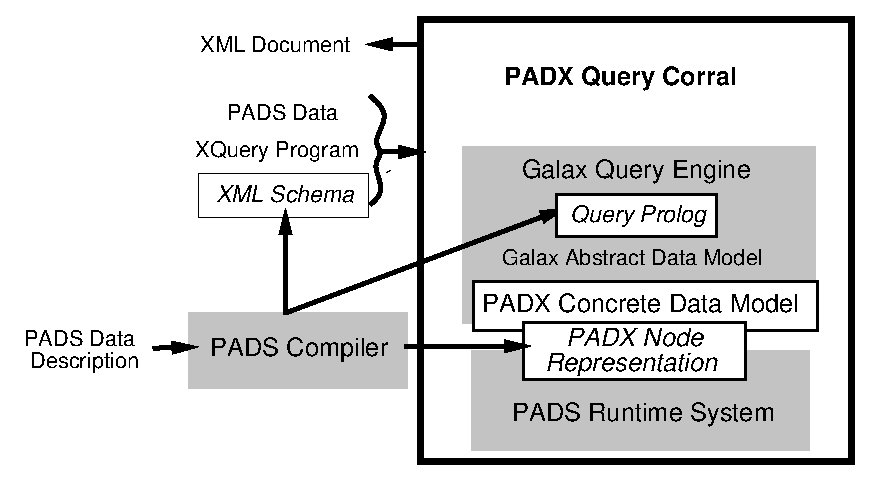
\epsfig{file=padx-arch.ps,width=0.47\textwidth}
\end{center}
\caption{\padx{} Architecture}
\label{figure:padx-arch}
\end{figure}

Put the pieces all together.  Sythesis of the two systems here. 
(Symbiotic)

\subsection{Virtual XML view of PADS data}

Embedding of PADS types in XML Schema.  One-to-one mapping from
PADS compound types to XML Schema complex types.  One-to-one mapping
from PADS base types to XML Schema simple types.  Field in compound
types are realized as local elements in XML Schema. 

All the compound types are annotated with an optional parse-descriptor
(absent if no errors occured).  Allows users to query error
structures, which may be most important data.  Other types annotated
with corresponding fields from PADS rep, e.g., arrays have a length. 

Extra level of indirection in representation of arrays---wrap each
item in an element. 

Extra level of indirection for base types: must contain the value of
the base type and an optional parse-descriptor, if an error has
occurred. 

We don't take complete advantage of XML Schema, e.g., Penum types
could be modeled by XML Schema enumeration simple types, but currently
unsupported.

Generated XML Schema.

\begin{figure*}
\begin{small}
\begin{code}
<xs:schema targetNamespace="file:sirius.p"
           xmlns="file:sirius.p"
           xmlns:xs="http://www.w3.org/2001/XMLSchema"
           xmlns:p="http://www.padsproj.org/pads.xsd">
<xs:import namespace = "http://www.padsproj.org/pads.xsd".../>
...
<xs:complexType name="\kw{order_header_t}">
 <xs:sequence>
  <xs:element name="order_num" type="p:val_Puint32"/>
  <xs:element name="att_order_num" type="p:val_Puint32"/>
  <xs:element name="ord_version" type="p:val_Puint32"/>
  <!-- More local element declarations -->
  <xs:element name="pd" type="\kw{p:PStruct_pd}" minOccurs="0"/>
 </xs:sequence>
</xs:complexType>
<!-- More complex type declarations -->
<xs:complexType name="\kw{orders_t}">
 <xs:sequence>
  <xs:element name="\kw{elt}" type="order_t" maxOccurs="unbounded"/>
  <xs:element name="\kw{length}" type="p:Puint32"/>
  <xs:element name="\kw{pd}" type="\kw{p:Parray_pd}" minOccurs="0"/>
 </xs:sequence>
</xs:complexType>
...
</xs:schema>
\end{code}
\end{small}
\caption{Fragment of XML Schema for \dibbler{} \pads{} description.}
\label{figure:dibbler-schema}
\end{figure*}

``Error-aware'' mapping from PADS type system to isomorphic XML
Schema. 
\begin{small}
\begin{code}
<xs:complexType name="\kw{val_Puint32}">
  <xs:choice>
   <xs:element name="val" type="p:Puint32"/>
   <xs:element name="pd" type="p:Pbase_pd"/>
  </xs:choice>
</xs:complexType>
<xs:complexType name="\kw{Pbase_pd}">
 <xs:sequence>
   <xs:element name="\kw{pstate}"  type="p:Pflags_t"/>
   <xs:element name="\kw{errCode}" type="p:PerrCode_t"/>
   <xs:element name="\kw{loc}"     type="p:Ploc_t"/>
 </xs:sequence>
</xs:complexType>
\end{code}
\end{small}

Example of query that uses generated schema.
\begin{small}
\begin{code}
declare namespace p = "http://www.padsproj.org/pads.xsd";
import schema default element namespace "file:sirius.p"
  schemaLocation "file:/somewhere/sirius.xsd";

$pads/p:Psource/orders/elt[events/elt[1]
  [tstamp >= xs:dateTime("2004-10-01:00:00:00") and 
   tstamp < xs:date("2004-11-01:00:00:00") ]]
\end{code}
\end{small}

\subsection{Physical Data Model}

Implementation of Galax's Abstract Tree Model.

Minimum necessary to implement Galax DM:

1. Generic implementations of the DM accessors: axis::node-test(), children(),
   attributes(), name(), etc. 

2. On PADX-side, we have a virtual handle for each node in the XML
   tree--we call that a node rep.  Node rep contains pads handle
   (maintains state for PADS parser); type-specific vtable of DM
   accessors; other stuff...

   Give example of vtable for event\_t and possibly code for
   kthChildByName. 

When to actually read from PADS data?

Options: 

1. Bulk read: Materialize entire PADS representation, populate all of the PADS
reps.  Then PADX DM lazily invoked the DM accessors over this data.
Problem: if data is big, it's all sitting in memory, even if the query
only touches a fragment of the virtual XML tree.

2. Smart read: 

Many common queries permit sequential, streamed access to underlying
XML source.  Give an example.  

Smart node rep, preserves meta-data about previously read records, but
re-uses memory for reading next item.  This rep permits multiple scans
of input (semantic problem is that DM must preserve node identity),
but slowly. 

Heuristic: records are a good level of granularity to read.   Each
smart node corresponds to one record.  When next smart node is
accessed, a little meta-data is preserved: the node rep and the
records location in the file (so we can re-read it if necessary).

3. Linear read: same as smart but does not preserve meta-data.
   Does not permit multiple scans of data source. 

Put in PADX signatures for constructing a new node and accessing
kthChild. 

\section{Performance}
\label{section:performance}

\subsection{Materialization and Loading}

Hypothesis: bulk loading should not scale for increasing document size
(limits of main memory).  Show that smart/linear does scale.

\subsection{Querying}

Give examples of queries that analyst cares about. 

Example of query that can be evaluated in single scan over data
source, but is currently not 

Database person would balk at this point!  Why aren't you just loading
this data into a real database, building indices and getting good
query performance?  B/c data is ephmeral, queries are ephmeral, but
analyst/programmer should profit from disciplined access/querying of
their data.  Don't abandon them to Perl. 

\section{Related Work}
\label{section:relatedwork}

DFDL. Contivo. 

\section{Future Work and Discussion}
\label{section:future}
Open problem: give result of XQuery and its corresponding type,
serialize result back into PADS rep.  How are the syntactic
constraints for the new values expressed?  Tool could pick default
delimiters automatically. 

Open problem: given an arbitrary PADS type, permit skipping and
reading at arbitrary positions within the data source. 

Big open problem: Given arbitrary XQuery expression, determine whether
it can be evaluated in single scan over data.  

\bibliographystyle{abbrv}
\small
\bibliography{../pldi/pads} 

\end{document}

\subsubsection{XML Generation}
\pads{} also supports converting ad hoc data into XML by providing a canonical mapping from \pads{} descriptions into XML.  This mapping is quite natural, as both \pads{} and XML are languages for describing semi-structured data.
One interesting aspect of the mapping is that we embed not just the in-memory representation of \pads{} values, but also the parse descriptors in cases where the data was buggy.  This choice allows users to explore the error portions
of their data sources, which can be the most interesting parts of the data.
Given a \pads{} specification, the \pads{} compiler generates an XML Schema describing the canonical embedding for that data source.  As an example, 
the following is the portion of the generated XML Schema for the \cd{eventSeq} type in the \dibbler{} data description.

The \pads{} compiler generates a \cd{write_xml_2io} function for each type, an example of which is shown in \figref{figure:library}.  Given a specification of the top level type, \pads{} can also automatically generate a conversion program, the output of which conforms to the generated XML Schema.

\subsection{Queries}
Our final use-scenario is querying data.
Given a data source, a natural desire is to ask questions about the data, a desire which led to SQL and its many variants for relational data and XQuery for XML data~\cite{boag03XQueryDraft}.  Analysts working with ad hoc data would also like to query their
data, but the lack of tools generally means they code their queries in an imperative fashion in languages such as \textsc{awk}, \perl{}, or \C{}.
Indeed, the analyst working with the \dibbler{} data took this approach.
He coded queries such as ``Select all orders starting within a certain time window," ``Count the number of orders going through a particular state," and ``What is the average time required to go from a particular state to another
particular state" in a mixture of \textsc{awk} and \textsc{perl}.  He was
able to get the answers to his questions, but he had to code the queries explicitly, and the query-related code ended up embedded in his already-brittle parsing code.

We wanted to support declarative querying over ad hoc sources, but we didn't want to invent an entirely new query language, which led us to examine existing languages.  Because XQuery is designed to manipulate semi-structured data, its expressiveness matched our data sources well.  We were able to code all the \dibbler{}-related queries in XQuery.  For example, the XQuery
\begin{code}
\begin{small}
{ $sirius/sirius/order[event[1]
    [timeStamp >= xs:date("2002-04-14") and 
     timeStamp <= xs:date("2002-05-25") ]] }
\end{small}
\end{code}
asks for all orders starting within the given time window.  

Happy with XQuery's expressiveness, we worked with the designers of the Galax~\cite{galax} open-source implementation of XQuery to define a data API~\cite{galaxmanual}. 
This API presents the source as a tree to Galax. With this architecture, Galax can incorporate any data source accessible through an instance of the data API.  We then extended the \pads{} system to produce such instances.  We were able to define the bulk of the API generically, having to generate on a per type basis only a handful of functions. 
\figref{figure:library} contains the key generated functions for the \cd{entry_t} type from the \dibbler{} data.    The  \cd{node_new} function creates a node in the tree representation of the data, storing the supplied name, mask, parse descriptor, and in-memory representation.  It makes the argument node the parent of the newly created node.
The \cd{node_kthChild} function takes a tree
corresponding to an \cd{entry_t} node and a child index and returns the appropriate child.  For the \cd{entry_t} type, possible children are the header, the event sequence, or a parse descriptor. 
At the moment, it is possible to use the resulting system to query ad hoc data sources that can be loaded entirely into memory, and a version that allows the data to be read lazily is well underway.
How best to optimize Xqueries over ad hoc data sources is an open research area.


\begin{figure}
\begin{small}
\begin{code}
<xs:schema targetNamespace="http://www.padsproj.org/pads.xsd"
           xmlns:p="http://www.padsproj.org/pads.xsd"
	   xmlns:xs="http://www.w3.org/2001/XMLSchema">
<xs:complexType name="\kw{val_Puint32}">
  <xs:choice>
   <xs:element name="val" type="p:Puint32"/>
   <xs:element name="pd" type="p:Pbase_pd"/>
  </xs:choice>
</xs:complexType>
...
<xs:complexType name="\kw{Pstruct_pd}">
<xs:sequence>
<xs:element name="\kw{pstate}"  type="p:Pflags_t"/>
<xs:element name="\kw{nerr}"    type="p:Puint32"/>
<xs:element name="\kw{errCode}" type="p:PerrCode_t"/>
<xs:element name="\kw{loc}"     type="p:Ploc_t"/>
</xs:sequence>
</xs:complexType>

<xs:complexType name="\kw{Parray_pd}">
<xs:sequence>
<xs:element name="{pstate}"   type="p:Pflags_t"/>
<xs:element name="nerr"       type="p:Puint32"/>
<xs:element name="errCode"    type="p:PerrCode_t"/>
<xs:element name="loc"        type="p:Ploc_t"/>
<xs:element name="\kw{neerr}" type="p:Puint32"/>
<xs:element name="\kw{firstError}" type="p:Puint32"/>
</xs:sequence>
</xs:complexType>
...
</xs:schema>
\end{code}
\end{small}
\caption{Fragment of XML Schema for \dibbler{} \pads{} description.}
\label{figure:dibbler-schema}
\end{figure}
